\documentclass{article}
\usepackage[utf8]{inputenc} %кодировка
\usepackage[T2A]{fontenc}
\usepackage[english,russian]{babel} %русификатор 
\usepackage{mathtools} %библиотека матеши
\usepackage[left=1cm,right=1cm,top=2cm,bottom=2cm,bindingoffset=0cm]{geometry} %изменение отступов на листе
\usepackage{amsmath}
\usepackage{graphicx} %библиотека для графики и картинок
\graphicspath{}
\DeclareGraphicsExtensions{.pdf,.png,.jpg}
\usepackage{subcaption}
\usepackage{pgfplots}
\usepackage{array}
\usepackage{pgfplots}
\usepackage{float}
\pgfplotsset{compat=1.16}

\begin{document}
% НАЧАЛО ТИТУЛЬНОГО ЛИСТА
\begin{center}
    \Large
    Федеральное государственное автономное \\
    образовательное учреждение высшего образования \\ 
    «Научно-образовательная корпорация ИТМО»\\
    \vspace{0.5cm}
    \large
    Факультет программной инженерии и компьютерной техники \\
    Направление подготовки 09.03.04 Программная инженерия \\
    \vspace{1cm}
    \Large
    \textbf{Отчёт по лабораторной работе №4} \\
    По дисциплине «Математическая статистика» (четвёртый семестр)\\
    Исследование распределения случайной величины\\
    \large
    \vspace{8cm}

    \begin{minipage}{.33\textwidth}
    \end{minipage}
    \hfill
    \begin{minipage}{.4\textwidth}
    
        \textbf{Студент}: \vspace{.1cm} \\
        \ Дениченко Александр\\
        \ Разинкин Александр\\
        \ Соколов Анатолий\\
        \textbf{Практик}:  \\
        \ Милованович Екатерина Воиславовна
    \end{minipage}
    \vfill
Санкт-Петербург\\ 2024 г.
\end{center}

% КОНЕЦ ТИТУЛЬНОГО ЛИСТА 
\newpage
\section*{Цель работы:}
\large

На основании анализа опытных данных

4. Проверить статистическую гипотезу о виде закона распределения генеральной совокупности.
\section{Интервальный ряд}
По условию нам дано n = 100. k - число интервалов:
\begin{equation*}
    k = \sqrt{100} = 10
\end{equation*}
\begin{table}[h]
    \centering
    \begin{tabular}{|*{10}{c|}}
        \hline
        -0.499 & 1.683 & 2.247 & 1.444 & -0.418 & -2.977 & -0.968 & -0.308 & -1.816 & -0.446 \\
        \hline
        1.627 & 1.555 & 0.310 & -0.074 & 1.414 & 1.007 & 0.555 & 0.003 & -2.789 & 0.005 \\
        \hline
        -0.239 & -1.050 & 1.991 & -0.362 & -0.847 & 0.884 & 0.759 & -1.406 & 0.262 & -0.206 \\
        \hline
        -0.961 & 0.096 & -0.119 & -0.777 & 0.166 & -0.405 & -0.572 & 1.624 & 0.119 & 0.049 \\
        \hline
        -0.152 & 0.251 & -0.272 & -0.250 & -0.048 & -2.619 & 1.158 & 0.139 & 0.332 & 0.926 \\
        \hline
        0.350 & 0.033 & 0.478 & 0.637 & -0.033 & -0.319 & 0.570 & -0.837 & -0.413 & -1.640 \\
        \hline
        -0.795 & -0.015 & 1.774 & -1.568 & 0.302 & -1.120 & -0.917 & -0.091 & 1.118 & 0.277 \\
        \hline
        -0.622 & -0.554 & -0.470 & 0.700 & -0.656 & 1.460 & 1.701 & 0.630 & -0.700 & -0.674 \\
        \hline
        1.429 & -1.163 & -0.925 & 0.973 & -0.052 & 0.409 & -0.024 & 0.384 & -0.350 & 0.203 \\
        \hline
        -2.084 & 0.100 & 0.001 & -0.070 & 0.773 & 1.132 & -0.769 & -0.609 & 1.816 & 1.307 \\
        \hline
    \end{tabular}
    \caption{Данные}
\end{table}
\\
На уровне значимости $\alpha = 0.05$ проверим гипотезу $H_0$ о нормальном распределении генеральной совокупности против конкурирующей гипотезы
$H_1$ о том, что она так не распределена. Используем критерий согласия Пирсона:
\[\chi^2 = \sum\frac{(n_i-n_i')^2}{n_i'}\]
\begin{center}
    \begin{table}[h]
        \centering
        \begin{tabular}{|*{11}{c|}}
            \hline
            $x_i^*$& $n_i$ &$x_i^*n_i$ &$x_i^{*2}n_i$\\
            \hline
            -2,725&	3	&-8,175	&22,277\\
            \hline
            -2,175&	1&	-2,175&	4,731\\
            \hline
            -1,625&	4	&-6,5&	10,5625\\
            \hline
            -1,075 & 9 & -9,675 & 10,400625 \\
            \hline
            -0,525 & 21 & -11,025 & 5,788125 \\
            \hline
            0,025 & 27 & 0,675 & 0,016875 \\
            \hline
            0,575 & 14 & 8,05 & 4,62875 \\
            \hline
            1,125 & 8 & 9 & 10,125 \\
            \hline
            1,675 & 11 & 18,425 & 30,861875 \\
            \hline
            2,225 & 2 & 4,45 & 9,90125\\
            \hline
            Суммы &100& 3.05& 109.29\\
            \hline
        \end{tabular}
    \end{table}
\end{center}
Выборочное среднее: 
\[\overline{X} = \frac{\sum x_i^*n_i}{n} = 0,0305\]
Выборочная дисперсия:
\[S^2 = \frac{\sum x_i^{*2}n_i}{n} - \overline{X}^2 = 1,092\]
Выборочное отклонение:
\[\sigma = \sqrt{S^2} = \sqrt{1,092} = 1,045\]
По причине большого объёма выборки его исправлением можно пренебречь.
Теоретические частоты рассчитываются по формуле:
\[n_i' = \frac{h\cdot n}{\sigma}\cdot f(z_i)\]
\[f(z) = \frac{1}{\sqrt{2\pi}}e^{-\frac{z^2}{2}}\]
Знакомая функция Гаусса 
\[z_i = \frac{x_i^* - \overline{X}}{\sigma}\]

\begin{center}
    \begin{table}[h]
        \centering
        \begin{tabular}{|*{5}{c|}}
            \hline
            $x_i^*$& $n_i$ &$z_i$ &$f(z_i)$& $n_i'$\\
            \hline
            -2,725 & 3 & -2,637 & 0,012 & 0,65 \\
            \hline
            -2,175 & 1 & -3,126 & 0,003 & 0,16 \\
            \hline
            -1,625 & 4 & -2,555 & 0,015 & 0,8 \\
            \hline
            -1,075 & 9 & -1,029 & 0,235 & 12,37 \\
            \hline
            -0,525 & 21 & -0,502 & 0,352 & 18,51 \\
            \hline
            0,025 & 27 & 0,024 & 0,399 & 20,99 \\
            \hline
            0,575 & 14 & 0,55 & 0,343 & 18,05 \\
            \hline
            1,125 & 8 & 1,077 & 0,223 & 11,76 \\
            \hline
            1,675 & 11 & 1,603 & 0,11 & 5,81 \\
            \hline
            2,225 & 2 & 2,129 & 0,041 & 2,18\\
            \hline
        \end{tabular}
    \end{table}
\end{center}
Cледует объединить интервалы с малыми частотами.
\begin{center}
    \begin{table}[h]
        \centering
        \begin{tabular}{|*{5}{c|}}
            \hline
            $n_i$ &$n_i'$\\
            3 & 0,65 \\
            \hline
            1 & 0,16 \\
            \hline
            4 & 0,8 \\
            \hline
            9 & 12,37 \\
            \hline
            21 & 18,51 \\
            \hline
            27 & 20,99 \\
            \hline
            14 & 18,05 \\
            \hline
            8 & 11,76 \\
            \hline
            11 & 5,81 \\
            \hline
            2 & 2,18\\
            \hline
        \end{tabular}
        \caption{До объединения}
    \end{table}
\end{center}
\begin{center}
    \begin{table}[H]
        \centering
        \begin{tabular}{|*{3}{c|}}
            \hline
            $n_i$ &$n_i'$& $\frac{(n_i-n_i')^2}{n_i'}$\\
            \hline
            8 & 1,61 & 25,3615528 \\
            \hline
            9 & 12,37 & 0,918100243 \\
            \hline
            21 & 18,51 & 0,334959481 \\
            \hline
            27 & 20,99 & 1,720824202 \\
            \hline
            14 & 18,05 & 0,908725762 \\
            \hline
            8 & 11,76 & 1,202176871 \\
            \hline
            13 & 7,99 & 3,141439299\\
            \hline
             Сумма& &33,58777865\\
             \hline
        \end{tabular}
        \caption{После объединения}
    \end{table}
\end{center}
\[\chi^2_{\text{кр}} = 9.5\]
\[\chi^2_{\text{набл}} \approx 33,58777865 > \chi^2_{\text{кр}}\]
\section*{Вывод}
На уровне значимости 0,05 гипотезу $H_0$ о нормальном распределении генеральной совокупности отвергаем.

\end{document}
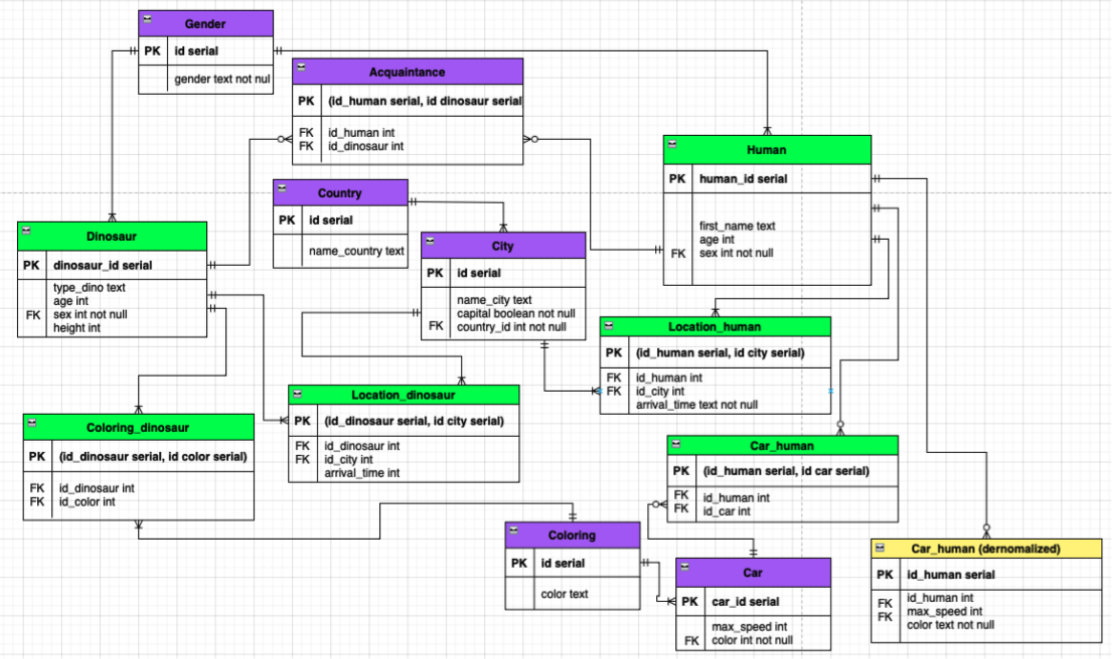
\includegraphics[width=.9\textwidth]{123}